\documentclass{article}
\usepackage{graphicx} % Required for inserting images
\usepackage{amsmath,amssymb,amsxtra,tikz,stackengine,bm,mathrsfs,bbm,tikz-cd,comment,combelow,amsopn}
\usepackage{amsthm}
\usetikzlibrary{arrows.meta}
\usepackage{pgfplots}
\pgfplotsset{compat=1.18}
\usepackage{amscd}
\usepackage{url}

\title{Dehn Twists and Deformation Spaces.}
\author{Tanya Firsova, Mikhail Mazin}
\date{August 2026}

\begin{document}
\begin{center}
{\large Tanya Firsova and Mikhail Mazin}
\end{center}
\newcommand{\aaa}{\mathfrak{a}}
\newcommand{\cc}{\mathfrak{c}}
\newcommand{\bb}{\mathfrak{b}}
\newcommand{\C}{\mathbb{C}}
\newcommand{\CP}{\mathbb{CP}^1}
\newcommand{\Z}{\mathbb{Z}}
\newcommand{\W}{\mathcal{W}}
\newcommand{\U}{\mathcal{U}}
\newcommand{\V}{\mathcal{V}}
\newcommand{\D}{\mathcal{D}}
\newcommand{\X}{\mathcal{X}}
\newcommand{\Q}{\mathcal{Q}}
\newcommand{\M}{\mathcal{M}}
\newcommand{\Pf}{\mathcal{P}}
\newcommand{\Def}{\mathcal{D}}
\renewcommand{\S}{\mathbb{S}}
\newcommand{\e}{\varepsilon}
\newcommand{\s}{\mathfrak{s}}
\newcommand{\Per}{\operatorname{Per}}
\newcommand{\Mod}{\operatorname{Mod}}
\newcommand{\Mapp}{\operatorname{MCG}}
\newcommand{\Teich}{\operatorname{Teich}}

%\newtheorem*{theorem*}{Theorem}

\newtheorem{theorem}{Theorem}[section]
\newtheorem{lemma}[theorem]{Lemma}
\newtheorem{proposition}[theorem]{Proposition}
\newtheorem{corollary}[theorem]{Corollary}
\newtheorem{conjecture}[theorem]{Conjecture}
\newtheorem{question}[theorem]{Question}

\theoremstyle{definition}
\newtheorem{definition}[theorem]{Definition}
\newtheorem{example}[theorem]{Example}
\newtheorem{construction}[theorem]{Construction}

\theoremstyle{remark}
\newtheorem{remark}[theorem]{Remark}


\numberwithin{equation}{section}
\section{Introduction}

J. Milnor \cite{Milnor} studied the space ${\mathcal M}_2^{cm}$ of equivalence classes of quadratic rational maps with marked critical points. The maps are equivalent if they are conjugate by a M\"obius transformation. Each representative has two critical points $c_1,c_2$. J. Milnor has shown that ${\mathcal M}_2^{cm}$ is isomorphic to $\C^2.$ He identified and studied the following 1-dimensional families:
$$\Per_n = \{ f\in\mathcal{M}^{cm}_2 :\, f^{\circ k}(c_1) = c_1 \quad \mbox{if and only if}\quad  n|k\}.$$
Let $v=f(c_2),$ define
$$
\Per'_n=\{f\in \Per_n: \, v\neq f^k(c_1), k=0,1,\dots,(n-1)\}.
$$ 

$\Per'_n$ can be naturally embedded in the moduli space $\M_{0,n+1}$ of a sphere with $(n+1)$-marked points, by marking the critical cycle and the extra critical value. Each component of the embedding has a natural cover, called the \textit{deformation space}, in the Teichm\"uller space (see \cite{HK,FKS}).

The \textit{Teichm\"uller space} $\Teich(P)$ of the sphere with points in the finite set $P$ marked is the space of equivalence classes of orientation-preserving homeomorphisms $\phi:(\S^2, P)\to (\C{\mathbb P}^1, P')$. Two such homeomorphisms $\phi_1:(\S^2, P)\to (\C{\mathbb P}^1, P')$ and $\phi_2:(\S^2, P)\to (\C{\mathbb P}^1, P'')$ are equivalent if there exist an orientation-preserving homeomorphism $\beta:({\mathbb S}^2, P)\to ({\mathbb S}^2, P)$, isotopic to the identity relative to $P$, and a M\"{o}bius transformation $\alpha$, such that the following diagram commutes: 
\[
\begin{tikzcd}
(\S^2, P) \arrow{r}{\phi_1} \arrow{d}{\beta}  & (\C{\mathbb P}^1, P') \arrow{d}{\alpha}  \\
(\S^2, P) \arrow{r}{\phi_2} &  (\C{\mathbb P}^1, P'')
\end{tikzcd}
\]

%We will often suppress the sphere in the argument $\Teich(P)=\Teich(\S^2,P),$ since we are not going to consider Teichm\"uller spaces of other surfaces. 

Deformation spaces were defined and studied by A. Epstein, see, for example, \cite{HK,FKS}.
Let $f:{\mathbb S}^2\to {\mathbb S}^2$ be a branched cover and $V(f)$ be the  set of critical values of $f$. Let $A, B\subset {\mathbb S}^2$ be finite subsets such that 
$$
A\cup f(A)\cup V(f)\subset B.
$$

Since $V(f)\subset B$, the map $f:{\mathbb S}^2\setminus f^{-1}(B)\to {\mathbb S}^2\setminus B$ is an (unbranched) covering map. By changing the complex structure on $({\mathbb S}^2, B)$ and applying the pull-back, one obtains a complex structure on $({\mathbb S}^2, f^{-1}(B))$. Then by erasing points in $f^{-1}(B)\backslash A$ and extending the complex structure, we obtain the complex structure on $({\mathbb S}^2, A)$. This process induces the pull-back map 
 $$f^*: \Teich(B) \to \Teich(A),$$
 where $\Teich (A)$, $\Teich (B)$ are the Teichm\"{u}ller spaces of the sphere with sets $A$, $B$ marked.
 Since $A\subset B$, the forgetful map is also well-defined:
 $$i_*:\Teich( B)\to \Teich(A).$$

\begin{definition}
The deformation space $\Def_f$ is defined as follows:  
$$\Def_f:=\{\tau\in \Teich (B) :\quad f^*\tau = i_*\tau\}.$$ 
\end{definition}

The map $F:(\CP, A')\to(\CP, B')$ is \textit{Hurwitz equivalent} to $f$ if there exist orientation-preserving homeomorphisms of pairs $\psi:(\S^2,A)\to(\CP, A')$, $\phi:(\S^2,B)\to(\C{\mathbb P}^1, B'),$ such that $F\circ \psi=\phi \circ f$. The space of isotopy classes $[\psi,\phi,F]$ of maps Hurwitz equivalent to $f$ up to compositions with M\"obius transformations is isomorphic to the Teichm\"uller space $\Teich(B)$. By considering restrictions 
$[\psi|_A, \phi|_B, F]$ we obtain the moduli space $\W_f$ of maps Hurwitz equivalent to $f,$ together with the covering map $\omega:\Teich(B)\to\W_f$ (see \cite{HK}).

Let $h:(\S^2, B)\to (\S^2,B)$ be an orientation-preserving homeomorphism that fixes $B$ point-wise. The map $h$ is called \textit{liftable} if there is an orientation-preserving homeomorphism  $h':(\S^2, A)\to (\S^2,A)$ fixing $A$ point-wise such that $f\circ  h'=h\circ f.$ The lifting property descends to the pure mapping class group (see \cite{KPS}):
$$
L_f:=\{[h]\in \Mapp(B):\, h\, \mbox{is liftable}\}.
$$
All the mapping class groups that we consider fix marked set point-wise. We'll be omitting the word "pure" late on.
There is a well-defined action of the map $f$ on $L_f:$ 
$$f^*:L_f\to \Mapp(A),$$
$$f^*[h]=[h']$$

The group $L_f$ is a subgroup of finite index in $\Mapp(B),$ and the space $\W_f$ is a quotient of $\Teich(B)$ by the group of liftable elements $L_f$ (see \cite{K}). Note also that the forgetful map induces the action 
$$
i_*:\Mapp(B)\to \Mapp(A).
$$

An element of the mapping class group $[h]\in \Mapp(B)$ is called a \textit{self-equivalence} if $f^*[h]=i_*[h].$ We denote the group of self-equivalences by $G_f$, see \cite{FKS}. Note that $G_f\subset L_f.$ Choose a base point $t_0\in\D_f\subset\Teich(B)$ and let $v_0:=\omega(t_0)\in V_f\subset\W_f.$ Then one gets an isomorphism between $\pi_1(\W_f,v_0)$ and $L_f,$ and one can think about $G_f$ as a subgroup of $\pi_1(\W_f,v_0).$ Let $\D_f^0$ be the connected component of the deformation space $\D_f$ containing $t_0,$ let $\V_f^0\subset\W_f$ be the image of $\D_f^0,$ and $i_\V:\V_f^0\to\W_f$ be the embedding. The image of the fundamental group $G_0:=(i_\V)_*(\pi_1(\V_f^0,v_0))$ is a subgroup of $G_f$. If there is a self-equivalence $[h]\in G_f$ such that for all $n\in\Z_{>0}$ the element $[h^{\circ n}]$ does not belong to $G_0$, then the orbit of $\D_f^0$ under the action of $[h]$ on the components of $\D_f$ is infinite, \cite{HK}.

By taking $f\in \Per'_n,$ $A=\{c_1, f(c_1),\dots, f^{\circ(n-1)}(c_1)\}$, $B=A\cup\{v\},$ where $v=f(c_2)$ is the other critical value, we get a deformation space $\D_f\in \Teich(B).$ Note that in this case the sphere in the definition of the Teichm\"uller space is identified with $\CP$ and the class of the identity map $id:(\CP,B)\to (\CP,B)$ belongs to the fiber over $f\in\Per'_n\subset \M_{0,n+1}.$ %Note that in this case the base point $t_0\in\Teich(B)$ is fixed to be the class of the identity map $(\CP,B)\to (\CP,B)$ 
(see \cite{FKS}).
 
Following \cite{FKS}, we consider $n=4.$ The curve $\Per'_4$ is a sphere with $10$ points removed. By taking the normalization, $c_1=0$, $f(0)=\infty$, $f(\infty)=1,$ $f(1)=\rho$, we get a parametrization of $\Per'_4$ by $\rho$, and the following formula for $v$ (\cite{FKS}):
$$
v=1-\frac{(\rho^2+\rho-1)^2}{4(\rho-1)(2\rho^2-\rho)}.
$$

Hironaka and Koch (\cite{HK}) described $\W_f$ for $f\in \Per'_4$. By taking $A=\{0, 1, \infty, x\},$ $B=A\cup\{v\}$, and defining $F\in \W_f$ by the diagram
\[
\begin{tikzcd}
0 \arrow[d,"2"] & \infty \arrow[d] & 1 \arrow[d] & x \arrow[d] & c \arrow[d,"2"] \\
\infty & 1      & y & 0 & v
\end{tikzcd}
\]
where $0$ and $c$ are critical points, one gets a parametrization of the space $\W_f$ by the pair $(x,y).$ Function $F$ and the critical value $v$ are expressed as follows:
$$
F(z)=\frac{(z-x)(z-r)}{z^2},
$$
where $r=\frac{y}{x-1}+1,$ and
$$
v=1-\frac{(x^2-1+y)^2}{4x(x-1)(x+y-1)}.
$$

Note that the curve $\Per'_4$ is connected and isomorphic to $\V_f=\V_f^0\subset\W_f.$ See Figure \ref{fig: W_f} and \cite{HK} for details.

\section{The fundamental groups.}

\begin{figure}
\begin{center}
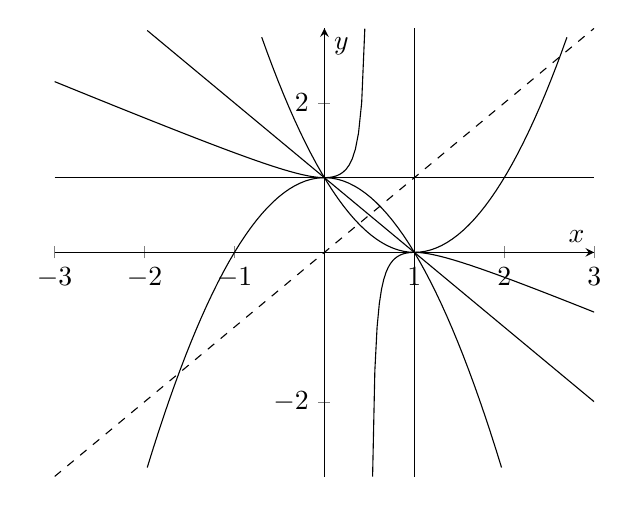
\begin{tikzpicture}
\begin{axis}[
  axis lines=middle, xlabel=$x$, ylabel=$y$,
  domain=-3:3, samples=100,
  xmin=-3, xmax=3,
  ymin=-3, ymax=3,
  restrict y to domain=-3:3,   % discards wild points instead of clipping lines
]
  \addplot[black] {0};      %\addlegendentry{$x^2$}
  \addplot[black] {1}; 
  \addplot[black] coordinates {(0,-3) (0,3)};
  \addplot[black] coordinates {(1,-3) (1,3)};
  \addplot[black] {1-x};
  \addplot[black] {x^2-2*x+1};
  \addplot[black] {1-x^2};
  \addplot[black, samples=100, domain=-3:0.4495] {(x^2-2*x+1)/(1-2*x)};
  \addplot[black, samples=100, domain=0.5359:3] {(x^2-2*x+1)/(1-2*x)};
  \addplot[black, dashed] {x};
\end{axis}
\end{tikzpicture}
\end{center}
\caption{$\mathcal{W}_f$ is the complement in $\C^2$ to the curves $y=0,$ $y=1,$ $x=0,$ $x=1,$ $x+y=1,$ $y=1-x^2,$ $y=x^2-2x+1,$ and $y-2xy=x^2-2x+1.$ The dashed line $y=x$ with ten punctures (seven of which are real and visible) is $\mathcal{V}_f=\omega(\mathcal{D}_f)$ the image of the deformation space under the covering $\omega:\Teich(B)\to\mathcal{W}_f.$}\label{fig: W_f}
\end{figure}

There are two projections $\rho_1,\rho_2: \mathcal{W}_f\to \CP\setminus\{0,1,\infty\}$ given by $\rho_1(x,y)=x$ and $\rho_2(x,y)=y.$ Consider the induced maps

\begin{equation*}
    (\rho_i)_*:\pi_1(\mathcal{W}_f,v_0)\to \pi_1(\CP\setminus\{0,1,\infty\},\rho_i(v_0)).
\end{equation*}

According to \cite{HK} we have $\pi_1(\mathcal{W}_f,v_0)\simeq L_f.$ Also, $\pi_1(\CP\setminus\{0,1,\infty\},\rho_i(v_0))$ is isomorphic to the mapping class group of the sphere with four marked points. According to \cite{HK}, under these identifications one has $(\rho_1)_*=f^*$ and $(\rho_2)_*=i_*.$ Our goal is to find an element $\gamma\in\pi_1(\mathcal{W}_f,v_0)$ such that $(\rho_1)_*\gamma=(\rho_2)_*\gamma$ and for any $n\in\Z_{>0}$ one has $\gamma^n\notin (i_\V)_*(\pi_1(\V_f,v_0)),$ where $i_\V:\V_f\to\W_f$ is the embedding. Since $\V_f$ is connected, we then obtain that the orbit of $\D_f^0$ under the action of $\gamma$ on the connected components of $\D_f$ is infinite.

Let $1\gg \e>0$ be a small positive number, and $a=0.5+\e.$ Set $v_0:=(a,a)\in\W_f$ to be the base point. In order to fix a base point $t_0\in\D_f,$ choose a path
$$
\zeta:[0,1]\to \Per'_4\simeq \V_f
$$
such that $\zeta(0)=f$ and $\zeta(1)=v_0$, let $\widetilde{\zeta}:[0,1]\to\D_f$ be its lift starting from the class of the identity map $\widetilde{\zeta}(0)=[id]\in\D_f\cap\omega^{-1}(f),$ and take $t_0:=\widetilde{\zeta}(1).$ 
%and fix a base point $t_0\in\omega^{-1}(v_0)\subset\Teich(B).$ Let $\D_f^0$ be the connected component of the deformation space $\D_f$ containing $t_0,$ and let 

%$$
%\phi:(\S^2,B)\to (\CP,\{0,1,\infty,y,v\})
%$$    

%be a representative of $t_0\in\Teich(B).$
%We pick $\e$ small enough so that $v_0$ is closer to $(0.5,0.5)$ than to the positive intersection of $y=1-x^2$ with the diagonal $y=x.$
\begin{definition}\label{def:alpha}
    Let $\alpha\in\pi_1(\W_f,v_0)$ be the class of the loop
$$
t \mapsto (0.5,0.5)+\e e^{2\pi i t}(1,1),\ t\in [0,1].
$$
\end{definition}

Let $(b,a)$ be the positive intersection of the line $y=a$ with the parabola $y=1-x^2,$ i.e. $b=\sqrt{1-a}.$

\begin{definition}\label{def:beta}
    Let $\beta\in\pi_1(\W_f,v_0)$ be the class of the loop defined as the concatenation of the following curves:
\begin{align*}
    &t\mapsto (t,a),\ t\in [a,b-\e],\\
    &t\mapsto (b+\e e^{2\pi i t},a),\  t\in [0.5,1],\\
    &t\mapsto (t,a),\ t\in [b+\e,1-\e],\\
    &t\mapsto (1+\e e^{2\pi i t},a),\ t\in [-0.5,0.5],\\
    &t\mapsto (-t,a),\ t\in [-(1-\e),-(b+\e)],\\
    &t\mapsto (b+\e e^{-2\pi i t},a),\ t\in [0,0.5],\\
    &t\mapsto (-t,a),\ t\in [-(b-\e),-a].
\end{align*}
In other words, the loop follows the real part of the line $\{y=a\}$ from $v_0=(a,a)$ almost to $(1,a),$ passing around the point $(b,a)$ in the complex part of $\{y=a\}$ counterclockwise, then goes counterclockwise full circle around $(1,a)$ in the complex part of $\{y=a\},$ and then retraces its steps back to $v_0$ (in particular, it goes clockwise around $(b,a)$ on the way back).
\end{definition}

The number $\e$ is chosen to be small enough so that $a<b-\e,$ $b+\e<1-\e,$ and the two loops described in the definitions above stay inside $\W_f$ and avoid the deleted curves. 

\begin{definition}
    Set $\gamma:=\beta\alpha\beta^{-1}\in\pi_1(\W_f,v_0).$
\end{definition}

\begin{lemma}
One has $(\rho_1)_*\gamma=(\rho_2)_*\gamma=1.$  
\end{lemma}

\begin{proof}
    Indeed, we have $(\rho_1)_*\alpha=(\rho_2)_*\alpha=1$ because $\{0.5\}$ is not a puncture in $\CP\setminus \{0,1,\infty\}.$ Hence, 
$$
(\rho_l)_*(\gamma)=(\rho_l)_*(\beta\alpha\beta^{-1})=1,
$$
for $l\in\{1,2\}.$
\end{proof}

\begin{theorem}
    For any $n\in \Z_{>0}$ one has $\gamma^n\notin (i_\V)_*(\pi_1(\V_f,v_0)).$
\end{theorem}

\begin{proof}
Following \cite{HK}, we introduce auxiliary spaces $(\X,x_0)$ and $(\Q,q_0)$ as follows:
    
\begin{align*}
    & (\X,x_0):=(\C^2\setminus \{x(x-1)y(y-1)(x+y-1)=0\},v_0),\\
    & (\Q,q_0):=(\C^2\setminus \{w(t-1)(w-t+1)=0\},(2a,a^2)).
\end{align*}

%\begin{remark}
%    There is a significant difference between \cite{HK} and its arxiv version \cite{HKarx}. For the description of $(\Q,q_0)$ one should follow \cite{HK}.
%\end{remark}

One gets the following maps:

$$
\begin{tikzcd}
    (\W_f,v_0) \arrow[r, "i_\W"] & (\X,x_0) \arrow[r, "\s"] & (\Q,q_0),
\end{tikzcd}
$$
where $i_\W:(\W_f,v_0)\to (\X,x_0)$ is the embedding, and $\s:(\X,x_0)\to (\Q,q_0)$ is given by 

$$
\s(x,y)=(x+y,xy).
$$

In other words, the map $\s$ factors $(\X,x_0)$ with respect to the symmetry $(x,y)\mapsto (y,x).$ To avoid confusion, we will use $(t,w)$ for coordinates in $\Q,$ so that $t=x+y$ and $w=xy.$ See Figure \ref{fig: X and Q} for illustration. It is immediate that 

$$
\Pf:=\overline{(\s\circ i_\W)(\V_f)}=\{(t,w)|w=t^2/4\}\subset\Q,
$$
where the closure is taken inside $\Q.$
\begin{figure}
\begin{center}
\begin{tikzpicture}[scale=0.8]
\begin{axis}[
  axis lines=middle, xlabel=$x$, ylabel=$y$,
  domain=-3:3, samples=100,
  xmin=-3, xmax=3,
  ymin=-3, ymax=3,
  restrict y to domain=-3:3,   % discards wild points instead of clipping lines
]
  \addplot[blue] {0};      %\addlegendentry{$x^2$}
  \addplot[red] {1}; 
  \addplot[blue] coordinates {(0,-3) (0,3)};
  \addplot[red] coordinates {(1,-3) (1,3)};
  \addplot[green] {1-x};
%  \addplot[black] {x^2-2*x+1};
%  \addplot[black] {1-x^2};
%  \addplot[black, samples=1000, domain=-3:0.4495] {(x^2-2*x+1)/(1-2*x)};
%  \addplot[black, samples=1000, domain=0.5359:3] {(x^2-2*x+1)/(1-2*x)};
  \addplot[black, dashed] {x};
\end{axis}
\end{tikzpicture}
\ 
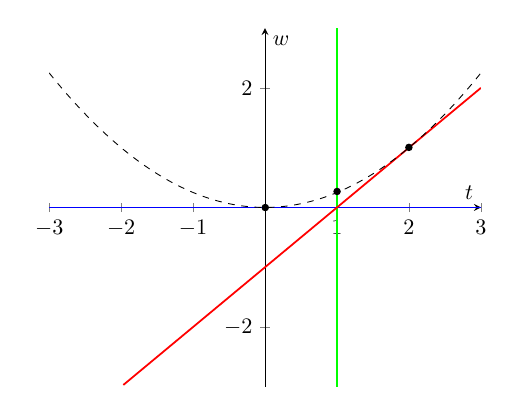
\begin{tikzpicture}[scale=0.8]
\begin{axis}[
  axis lines=middle, xlabel=$t$, ylabel=$w$,
  domain=-3:3, samples=100,
  xmin=-3, xmax=3,
  ymin=-3, ymax=3,
  restrict y to domain=-3:3,   % discards wild points instead of clipping lines
]
  \addplot[blue,thick] {0};      %\addlegendentry{$x^2$}
%  \addplot[black] {1}; 
%  \addplot[black] coordinates {(0,-3) (0,3)};
  \addplot[green,thick] coordinates {(1,-3) (1,3)};
  \addplot[red,thick] {x-1};
%  \addplot[black] {x^2-2*x+1};
%  \addplot[black] {1-x^2};
%  \addplot[black, samples=1000, domain=-3:0.4495] {(x^2-2*x+1)/(1-2*x)};
%  \addplot[black, samples=1000, domain=0.5359:3] {(x^2-2*x+1)/(1-2*x)};
  \addplot[black, dashed] {x^2/4};
\end{axis}
  \filldraw (3.43,2.845) circle [radius=0.5mm];
  \filldraw (4.57,3.1) circle [radius=0.5mm];
  \filldraw (5.71,3.8) circle [radius=0.5mm];
\end{tikzpicture}

\end{center}
\caption{The auxiliary spaces $\X$ (on the left) and $\Q$ (on the right). The dashed curve on the right is $\Pf=\overline{(\s\circ i_\W)(\V_f)}\subset\Q.$ Image-preimage pairs are color coded.}\label{fig: X and Q}
\end{figure}

Let $i_\Pf:\Pf\to\Q$ be the embedding. Note that $\Pf$ is isomorphic to $\C$ with three punctures: 
\begin{enumerate}
    \item point $(0,0),$ where $\Pf$ touches the line $\{w=0\},$
    \item point $(2,1),$ where $\Pf$ touches the line $\{w=t-1\},$ and
    \item point $(1,0.25),$ where $\Pf$ crosses the line $\{t=1\}.$
\end{enumerate}

Since $\Q$ is the complement to three concurrent lines in $\C^2,$ the fundamental group $\pi_1(\Q,q_0)$ is very well studied. It is generated by the classes $\aaa,\bb$ and $\cc,$ of loops going counterclockwise around the lines $\{t=1\},$ $\{w=t-1\},$ and $\{w=0\},$ respectively, subject to the relation $\cc\bb\aaa=\bb\aaa\cc=\aaa\cc\bb.$ 
More precisely, one can choose the generators $\aaa$ and $\bb$ to be the images of $\alpha$ and $\beta:$
\begin{align*}
&(\s\circ i_\W)_*(\alpha)=\aaa,\\
&(\s\circ i_\W)_*(\beta)=\bb,\\
\end{align*}
hence $(\s\circ i_\W)_*(\gamma)=\bb\aaa\bb^{-1}.$

Note that the defining representative of $\alpha$ can be moved homotopically to fit in the line $\{y=a\},$ and the defining representative for $\beta$ belongs to the line $\{y=a\}.$ Therefore, classes $\aaa$ and $\bb$ have representatives that lie in the line $\{w=at-a^2\}\subset\Q.$ Moreover, in $(\Q,q_0)$ the representatives of $\aaa$ and $\bb$ can be moved homotopically so that they follow the real part of the line $\{w=at-a^2\}$ from $q_0$ to the intersections with the lines $\{t=1\}$ and $\{w=t-1\}$ respectively, then go counterclockwise around these intersections, and then retrace back to $q_0.$ The class $\cc$ should then be defined by a representative that follows the real part of the line $\{w=at-a^2\}$ from $q_0$ to the intersection with the line $\{w=0\},$ bypassing the intersection with $\{t=1\}$ in the clockwise direction, then go around the intersection with $\{w=0\}$ counterclockwise, and then retrace back to $q_0.$ In this way, the element $z:=\aaa\cc\bb$ can be represented by a loop that goes around all three intersection points along a big circle in $\{w=at-a^2\}.$ See Figure \ref{fig: a,b,c} for an illustration.

On the other hand, one can consider the projection $\pi:\Q\to \CP\setminus \{\mathcal{A},\mathcal{B},\mathcal{C}\},$ where $\CP$ is identified with the space of lines passing through the point $(1,0)\in\C^2,$ and the points $\mathcal{A},\mathcal{B},\mathcal{C}$ correspond to the lines $\{t=1\},$ $\{w=t-1\},$ and $\{w=0\},$ respectively. In fact, it is a trivial fibration with fiber $\C^*$ (without the lines removed one would get the tautological bundle $\C^2\setminus \{(1,0)\}\to \CP,$ which is not trivial, but removing at least one fiber from it makes it trivial). In particular, one gets

\begin{equation}\label{eq:split}
\pi_1(\Q,q_0)\simeq \pi_1(\C^*)\times\pi_1(\CP\setminus \{\mathcal{A},\mathcal{B},\mathcal{C}\})\simeq  \Z\times F_2.
\end{equation}

Note that the restriction of $\pi$ to the line $\{w=at-a^2\}$ is an isomorphism onto $\CP\setminus \{\mathcal{A},\mathcal{B},\mathcal{C},\infty\},$ where $\infty$ corresponds to the line through $(1,0)$ parallel to $\{w=at-a^2\}.$ Hence, one gets that $\pi_*(\aaa\cc\bb)=\pi_*(\cc\bb\aaa)=\pi_*(\bb\aaa\cc)=1.$ However, Equation \ref{eq:split} implies that the kernel of $\pi_*$ is the center of $\pi_1(\Q,q_0)\simeq \Z\times F_2,$ which is the first factor $\Z.$ Hence, $\aaa\cc\bb,\cc\bb\aaa$ and $\bb\aaa\cc$ commute with the generators $\aaa,\bb,\cc$, which implies that $\aaa\cc\bb=\cc\bb\aaa=\bb\aaa\cc=z.$ Note that the images of $\aaa$ and $\bb$ generate $\pi_1(\CP\setminus \{\mathcal{A},\mathcal{B},\mathcal{C}\})\simeq F_2,$ therefore one has $\pi_1(\Q,q_0)\supset\langle \aaa,\bb\rangle\simeq F_2$ and one can write the splitting as $\pi_1(\Q,q_0)=\Z\times\langle \aaa,\bb\rangle.$ Since $\aaa,\bb,z$ also generate $\pi_1(\Q,q_0),$ it then follows that $z$ generates the center $\pi_1(\C^*)\simeq\Z.$

%It is well known that $z=cba=bac=acb$ generates the center of $\pi_1(\Q,q_0),$ which is isomorphic to $\Z$ (see \cite{HKarx} and references within, as well as \cite{B,FM}). 

\begin{figure}
\begin{center}
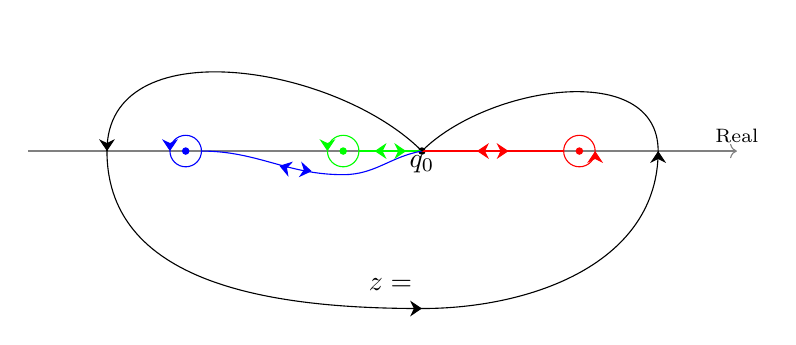
\begin{tikzpicture}[scale=1]
\draw[->, gray,thin] (-5,0)--(4,0); 

\filldraw (0,0) circle [radius=0.4mm]; 
\filldraw[red] (2,0) circle [radius=0.4mm]; 
\filldraw[green] (-1,0) circle [radius=0.4mm]; 
\filldraw[blue] (-3,0) circle [radius=0.4mm];

\draw[red] (2,0) circle [radius=2mm];
\draw[green] (-1,0) circle [radius=2mm];
\draw[blue] (-3,0) circle [radius=2mm];

\draw[red] [-{Stealth[length=1.5mm, width=2mm]}] (2.2,-0.01)--(2.2,0);
\draw[green] [-{Stealth[length=1.5mm, width=2mm]}] (-1.2,0.01)--(-1.2,0);
\draw[blue] [-{Stealth[length=1.5mm, width=2mm]}] (-3.2,0.01)--(-3.2,0);

\draw[red] (0,0)--(1.8,0);
\draw[green] (0,0)--(-0.8,0);
\draw[blue] (0,0) to[out=190,in=0] (-1,-0.3) to[out=180,in=0] (-2.8,0);
\draw (0,0) to[out=135,in=90] (-4,0) to[out=-90,in=180] (0,-2) to[out=0,in=-90] (3,0) to[out=90,in=45] (0,0);

\draw[red] [{Stealth[length=1.5mm, width=2mm]}-{Stealth[length=1.5mm, width=2mm]}] (0.7,0)--(1.1,0);
\draw[green] [{Stealth[length=1.5mm, width=2mm]}-{Stealth[length=1.5mm, width=2mm]}] (-0.2,0)--(-0.6,0);
\draw[blue] [-{Stealth[length=1.5mm, width=2mm]}] (-1.8,-0.19)--(-1.81,-0.187);
\draw[blue] [-{Stealth[length=1.5mm, width=2mm]}] (-1.41,-0.254)--(-1.4,-0.2555);
\draw [-{Stealth[length=1.5mm, width=2mm]}] (-4,0.001)--(-4,0);
\draw [-{Stealth[length=1.5mm, width=2mm]}] (3,-0.001)--(3,0);
\draw [-{Stealth[length=1.5mm, width=2mm]}] (-0.001,-2)--(0,-2);

\draw (4,0.2) node {\scriptsize Real};
\draw (0,-0.17) node {$q_0$};
\draw[blue] (-3.4,0.2) node {$\cc$};
\draw[red] (2.35,0.2) node {$\bb$};
\draw[green] (-1,0.35) node {$\aaa$};
\draw (-0.4,-1.7) node {$z=\aaa\cc\bb$};

\end{tikzpicture}
\end{center}
\caption{Representatives of the generators $\aaa,\bb,$ and $\cc$ of the group $\pi_1(\Q,q_0)$ inside the line $\{w=at-a^2\}.$ Note that in order to get the relation $\aaa\cc\bb=\cc\bb\aaa=\bb\aaa\cc$ one needs to step outside of the line $\{w=at-a^2\}$.}\label{fig: a,b,c}
\end{figure}

Note that the restriction $(\s\circ i_\W)|_{\V_f}$ is an isomorphism onto $\Pf$ with extra six points removed. It follows that the induced map from $\pi_1(\V_f,v_0)$ to $\pi_1(\Pf,q_0)$ is surjective, in particular, 
$$
(\s\circ i_\W)_*((i_\V)_*(\pi_1(\V_f,v_0)))=(i_\Pf)_*(\pi_1(\Pf,q_0)).
$$
Finally, one also gets
$$
(i_\Pf)_*(\pi_1(\Pf,q_0))=\langle \aaa,\bb^2,\cc^2\rangle.
$$
Indeed, one can choose the generators of $\pi_1(\Pf,q_0)$ in a way similar to the generators $\aaa,\bb,\cc,$ replacing the line $\{w=at-a^2\}$ with the parabola $\Pf=\{w=t^2/4\}:$ for $\aaa'\in\pi_1(\Pf,q_0)$ take the path starting at $q_0,$ following the real part of $\Pf$ to the intersection with $\{t=1\},$ then going around the intersection in the counterclockwise direction, and then retracing back to $q_0.$ Similarly, for $\bb'$ follow the real part of $\Pf$ to the intersection with $\{w=t-1\},$ go around it counterclockwise, and then retrace back. Finally, for $\cc'$ follow the real part of $\Pf,$ bypass the intersection with $\{t=1\}$ on the left (clockwise), proceed to the intersection with $\{w=0\},$ go around it counterclockwise, and then retrace back. 

One can then move homotopically these representatives inside $\Q$ to make them fit in the line $\{w=at-a^2\}:$ for $\aaa'$ one should project the representative to $\{w=at-a^2\}$ along the line $\{t=1\}$ or, more precisely, move it into the projection along the fibers of the projection. Note that the entire curve except for the tiny loop around $\{t=1\}$ will remain real all along the homotopy. Since the intersection of $\Pf$ with $\{t=1\}$ is transversal, the loop goes around $\{t=1\}$ once, therefore, $(i_\Pf)_*(\aaa')=\aaa.$ Similarly, for $\bb'$ one should project the representative along the line $\{w=t-1\},$ except that this time, because of the degree two tangency between $\Pf$ and $\{w=t-1\},$ the loop goes around $\{w=t-1\}$ twice, thus $(i_\Pf)_*(\bb')=\bb^2.$ Finally, for $\cc'$ one should project along the line $\{w=0\}.$ One should also be careful to keep bypassing the intersection with $\{t=1\}$ on the left. Again, due to the tangency between $\Pf$ and $\{w=0\}$ one obtains $(i_\Pf)_*(\cc')=\cc^2.$    


%However, while the intersection of $\Pf$ with the line $\{t=1\}$ is transversal, the intersections with the lines $\{w=t-1\}$ and $\{w=0\}$ are tangencies of order $2.$ Hence the images of the corresponding generators are $b^2$ and $c^2,$ while the image of the generator going around the intersection with $\{t=1\}$ is $a.$ 

%the loop on $\Pf$ going once, counterclockwise, around the respectively. puncture at $(0,0)$ goes around the line $\{w=0\}$ twice, because $\Pf$ and $\{w=0\}$ have a tangency of order $2$ and $(0,0).$ Hence its class in $\pi_1(\Q,q_0)$ is $c^2.$ Similarly, the class in $\pi_1(\Q,q_0)$ of the loop on $\Pf$ going around the puncture $(2,1)$ is $b^2.$ At the last puncture, $(1,0.25),$ $\Pf$ intersects the line $\{t=1\}$ transversely, hence the class of the corresponding loop is $a.$

We conclude that it suffices to show that for any $n\in\Z_{>0}$ one has 
$$
(\bb\aaa\bb^{-1})^n\notin \langle \aaa,\bb^2,\cc^2\rangle.
$$

For the sake of finding a contradiction, let us assume that 
$$
(\bb\aaa\bb^{-1})^n=\bb\aaa^n\bb^{-1}\in(i_\Pf)_*(\pi_1(\Pf,q_0))=\langle \aaa,\bb^2,\cc^2\rangle.
$$

Multiplying by $\bb^2\aaa\cc^2,$ one also gets 
\begin{align*}
\langle \aaa,\bb^2,\cc^2\rangle\ni\ &\bb^2\aaa\cc^2\cdot \bb\aaa^n\bb^{-1}=\bb^2\aaa\cc\cdot z \cdot \aaa^{n-1}\bb^{-1}\\
&=\bb\cdot z^2\cdot \aaa^{n-1}\bb^{-1}=\bb\aaa^{n-1}\bb^{-1}\cdot z^2.
\end{align*}

Repeating the above step $n$ times, one obtains:
$$
\langle \aaa,\bb^2,\cc^2\rangle\ni\ \bb\aaa^0\bb^{-1}\cdot z^{2n}=z^{2n}.
$$

However, Lemma $2.13$ in \cite{HK} states that the intersection of $(i_\Pf)_*(\pi_1(\Pf,q_0))=\s_*(\pi_1(\{x=y\}\cap \X,x_0))$ with the center of $\pi_1(\Q,q_0)$ is trivial. Contradiction.

%it is well known that the quotient $\pi_1(\Q,q_0)/\langle z\rangle$ is the free group generated by the images of $b$ and $c.$ Since $a=z(cb)^{-1},$ it also follows that the image of $\langle a,b^2,c^2\rangle$ is the subgroup generated by $cb,b^2,$ and $c^2,$ which is a free group with three generators (see e.g. \cite{HKarx}). Therefore the restriction of the projection to the subgroup $\langle a,b^2,c^2\rangle$ is injective, and $\langle a,b^2,c^2\rangle\cap \langle z\rangle=\{1\}.$ Contradiction.


\end{proof}

\section{The Dehn twists.}

In this section we study the mapping class corresponding to the element 
$$
\gamma=\beta\alpha\beta^{-1}\in \pi_1(\W_f,v_0)\simeq L_f
$$ 
constructed in the previous section. For convenience of the exposition, let us first consider the case when $f=v_0\in \Per'_4\simeq \V_f,$ so that the base point $t_0\in\D_f$ is the class of the identity map.

We start by showing that $\alpha$ corresponds to the class of the Dehn twist with respect to a certain closed simple loop $\varphi_\alpha:\S^1\to \CP\setminus \{0,1,\infty,y,v\}$. Since $\gamma$ is obtained from $\alpha$ by conjugating by $\beta,$ it follows that $\gamma$ corresponds to the Dehn twist with respect to the image of $\varphi_\alpha$ under a representative $f_\beta:\CP\setminus \{0,1,\infty,y,v\}\to \CP\setminus \{0,1,\infty,y,v\}$ of the mapping class corresponding to $\beta.$ For the background on the connections between Dehn twists, mapping class groups, and the elements of the fundamental groups of the moduli spaces, see \cite{B,FM}.

We proceed by first providing an explicit description of the loop $\varphi_\alpha,$ then constructing an explicit representative $f_\beta,$ and finally describing the image 
$$
f_\beta(\varphi_\alpha)=f_\beta\circ\varphi_\alpha:\S^1\to \CP\setminus \{0,1,\infty,y,v\}.
$$

Using the standard normalization, the moduli space $\M_B$ of five points on the Riemann sphere is given by
$$
\M_B\simeq \{B=\{0,1,\infty,y,v\}\subset \CP\}=\{y,v\in \C\setminus \{0,1\}|y\neq v\}.
$$

The projection $\W_f\to \M_B$ is then given by 
$$
(x,y)\mapsto \left(y,1-\frac{(x^2+y-1)^2}{4x(x-1)(x+y-1)}\right).
$$

The base point $(a,a)\in\W_f$ is then mapped to 
$$
\left(0,1,\infty,a,1-\frac{(a^2+a-1)^2}{4a(a-1)(2a-1)}\right)\in \M_B.
$$

Recall that $a=0.5+\e,$ where $\e$ is a small positive number. It follows then that $v_a:=1-\frac{(a^2+a-1)^2}{4a(a-1)(2a-1)}$ is a positive real number close to infinity.

The class $\alpha$ is defined using a loop going counterclockwise around the point $x=y=0.5$ inside the line $\V_f\subset\W_f$ (Definition \ref{def:alpha}). The image of this loop in the moduli space $\M_B$ corresponds to the point $y$ making a full counterclockwise turn around $0.5,$ while simultaneously the point $v$ makes a full counterclockwise turn around infinity. Since the trajectories don't intersect, the corresponding mapping class can be represented by the composition of Birman point-push maps corresponding to the two trajectories. However, the trajectory of $y$ is contractible, so the mapping class of the corresponding point-push map is trivial. The point-push map corresponding to $v$ going around infinity is equivalent to the Dehn twist corresponding to the simple closed curve that follows the trajectory except for going around $v_a$ on the right, so that the curve separates the marked points $v_a$ and $\infty$ from the marked points $0,1,$ and $y.$ More precisely, in the left-twist convention of \cite{FM}, it is the inverse of the corresponding Dehn twist. To be explicit, one can take
$$
\varphi_\alpha: t\to Re^{2\pi i t},\ t\in[0,1],
$$
where $R$ can be any real number such that $1<R<v_a.$ Of course, one can also take any other homotopy equivalent simple loop representative.

\begin{figure}
\centering
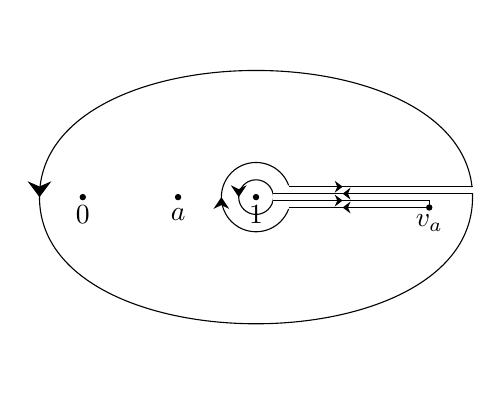
\begin{tikzpicture}[scale=1.1]
\filldraw (0,0) circle [radius=0.3mm];    
\filldraw (1.1,0) circle [radius=0.3mm];    
\filldraw (2,0) circle [radius=0.3mm];    
\filldraw (4,-0.12) circle [radius=0.3mm];    

\draw (0,-0.2) node {$0$};    
\draw (1.1,-0.2) node {$a$};    
\draw (2,-0.2) node {$1$};    
\draw (4,-0.3) node {$v_a$};    

\draw (2,0) circle [radius=2mm];
\draw (2,0) circle [radius=4mm];

\filldraw[white] (2.33,0) circle [radius=1.37mm];

\draw (4,-0.12)--(2.38,-0.12);
\draw (4.5,0.12)--(2.38,0.12);

%\draw (2,0) circle [radius=2.5cm];

\draw (4.5,0) to[out=90, in=90] (-0.5,0) to[out=-90,in=-90] (4.5,0);

\filldraw[white] (4.5,0.08) circle [radius=0.3mm];

\draw (4.5,0.04)--(2.2,0.04);
\draw (4,-0.12)--(4,-0.04)--(2.2,-0.04);

\draw [-{Stealth[length=1mm, width=1.5mm]}] (3.1,-0.12)--(3,-0.12);
\draw [-{Stealth[length=1mm, width=1.5mm]}] (2.9,0.12)--(3,0.12);
\draw [-{Stealth[length=1mm, width=1.5mm]}] (2.9,-0.04)--(3,-0.04);
\draw [-{Stealth[length=1mm, width=1.5mm]}] (3.1,0.04)--(3,0.04);
\draw [-{Stealth[length=1.5mm, width=2mm]}] (1.6,-0.01)--(1.6,0);
\draw [-{Stealth[length=1.5mm, width=2mm]}] (1.8,0.01)--(1.8,0);
\draw [-{Stealth[length=2mm, width=3mm]}] (-0.5,0.01)--(-0.5,0);
\end{tikzpicture}
    \caption{The image of the loop defining the class $\beta\in\pi_1(\W_f,v_0)$ in the moduli space $\M_B.$ Note that the points $0,1,\infty,$ and $a$ are fixed, and only one point $v$ is moving.}
    \label{fig:image of beta}
\end{figure}

We now move on to describing the image of the loop defining $\beta\in\pi_1(\W_f,v_0)$ (see Definition \ref{def:beta}) in the moduli space $\M_B.$ Lucky for us, the loop stays in the line $\{y=a\}$ the whole time, meaning that the only moving point in $\M_B$ is $v.$ Let us trace through the image of the curve following Definition \ref{def:beta} step-by-step:

\begin{enumerate}
    \item As $x$ travels along the real axis from $a$ to $b-\e,$ in the image $v$ will stay on the positive real semi-axis and move from $v_a$ near infinity to $1+\delta,$ where $\delta$ is a small positive real number.
    \item As $x$ makes a half circle around $(b,a)$ in the counterclockwise direction inside the line $\{y=a\}$, $v$ will make a full circle around $1$ in counterclockwise direction (it is not a perfect circle, and the end point is on the real line very close to $1+\delta,$ but not exactly $1+\delta$).
    \item As $x$ further travels along the real axis from $b+\e$ to $1-\e,$ in the image $v$ travels up the positive real axis almost to infinity.
    \item As $x$ goes around $(1,a)$ counterclockwise inside the line $\{y=a\},$ its image $v$ goes around infinity, also makes a full circle, counterclockwise.
    \item Finally, as $x$ retraces back to $(a,a),$ its image $v$ also retraces back the first three steps, going around $1$ clockwise and returning to $v_a.$
\end{enumerate}



See Figure \ref{fig:image of beta} for an illustration. Note that it suffices to determine the curve up to homotopy preserving the base point. See Figure \ref{fig:image of beta 2} for a nicer representative $\psi$ of the same homotopy class. 

\begin{figure}
\centering
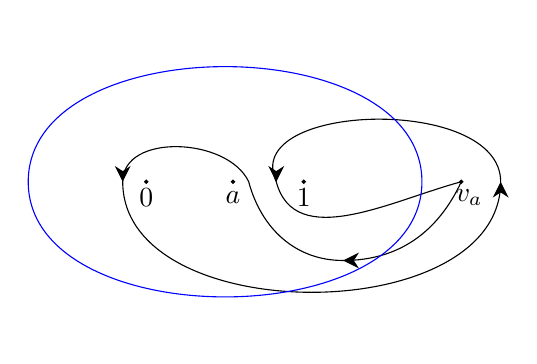
\begin{tikzpicture}[scale=1]
\filldraw (0,0) circle [radius=0.2mm];    
\filldraw (1.1,0) circle [radius=0.2mm];    
\filldraw (2,0) circle [radius=0.2mm];    
\filldraw (4,0) circle [radius=0.2mm];    

\draw (0,-0.2) node {$0$};    
\draw (1.1,-0.2) node {$a$};    
\draw (2,-0.2) node {$1$};    
\draw (4.1,-0.2) node {$v_a$};    

\draw (4,0) to[in=0,out=-115] (2.5,-1) to[out=180,in=-75] (1.3,0) to[out=115,in=90] (-0.3,0) to[out=-90,in=-90] (4.5,0) to[out=90,in=115] (1.65,0) to[out=-75,in=-165] (4,0);

\draw [-{Stealth[length=2mm, width=2mm]}] (2.51,-1)--(2.5,-1);
\draw [-{Stealth[length=2mm, width=2mm]}] (-0.3,0.01)--(-0.3,0);
\draw [-{Stealth[length=2mm, width=2mm]}] (4.5,-0.01)--(4.5,0);
\draw [-{Stealth[length=2mm, width=2mm]}] (1.65,0.01)--(1.65,0);

%\draw[blue] (1,0) circle [radius=2.5cm];
\draw[blue] (3.5,0) to[out=90,in=90] (-1.5,0) to[out=-90,in=-90] (3.5,0);
\end{tikzpicture}
    \caption{A nicer loop $\psi$ (in black) homotopy equivalent to the image of $\beta\in\pi_1(\W_f,v_0)$ from Figure \ref{fig:image of beta}. In blue is the loop $\varphi_\alpha$ such that the corresponding Dehn twist $T_{\varphi_\alpha}^{-1}$ represents the class $\alpha.$ In order to obtain the curve $\varphi_\gamma$ such that the Dehn twist $T_{\varphi_\gamma}^{-1}$ represents $\gamma,$ one should apply the Birman point-push map along $\psi$ to $\varphi_\alpha.$}
    \label{fig:image of beta 2}
\end{figure}

For a representative $f_\beta$ one can take the Birman point-push map corresponding to the loop $\psi.$ Equivalently, one can take a small tubular neighborhood of $\psi,$ let $\psi_L$ and $\psi_R$ be the two components of its boundary, with $\psi_R$ to the right of $\psi$ looking in the direction of the orientation of $\psi,$ and $\psi_L,$ respectively, to the left, and take $f_\beta$ to be the composition $T_{\psi_L}T_{\psi_R}^{-1},$ where $T_{\psi_R}$ and $T_{\psi_L}$ are the Dehn twists with respect to the loops $\psi_R$ and $\psi_L$ respectively.


Note that, in fact, $T_{\psi_R}$ is trivial in the mapping class group. Indeed, the loop $\psi_R$ is homotopy equivalent to a small loop around the marked point at $\infty,$ separating it from the other $4$ marked points. Therefore, one can simply take $\varphi_\gamma:=T_{\psi_L}(\varphi_\alpha),$ which provides an explicit description of the required loop. Note that one can also sketch $T_{\psi_L}(\varphi_\alpha)$ explicitly, but the rendering becomes somewhat messy, so we leave it to the reader's imagination.

Finally, in the general case when $f$ is not necessarily equal to $v_0,$ one should take a representative $\phi_{t_0}:(\CP,B)\to (\CP, \{0,1,\infty,a,v_a\})$ of the base point $t_0\in \omega^{-1}(v_0)\cap\D_f$ and apply the inverse map $\phi_{t_0}^{-1}$ to the whole construction. Note that a representative $\phi_{t_0}$ can also be constructed explicitly by applying point-push construction to the image of the curve $\zeta$ in the moduli space.


\begin{thebibliography}{99}
\bibitem{B} J. S. Birman, Braids, links, and mapping class groups, Ann. of Math. Stud., No. 82, Princeton University Press, Princeton, NJ; University of Tokyo Press, Tokyo, 1974.

\bibitem{FM} B. Farb, D. Margalit, A primer on mapping class groups, Princeton Math. Ser., 49 Princeton University Press, Princeton, NJ, 2012.

\bibitem{FKS} T. Firsova, J. Kahn, N. Selinger, 
On deformation spaces of quadratic rational functions.
Int. Math. Res. Not. IMRN 2023, no. 8, 6703--6738.

\bibitem{HK} E. Hironaka, S. Koch, A disconnected deformation space of rational maps. J. Mod. Dyn. 11 (2017), 409--423 (\url{https://websites.umich.edu/~kochsc/disconnected.pdf}).

%\bibitem{HKarx} E. Hironaka, S. Koch, A disconnected deformation space of rational maps, \url{https://arxiv.org/abs/1602.07378}.

\bibitem{K} S. Koch, Teichm\"uller theory and critically finite endomorphisms. Adv. Math. 248: (2013) 573–617.

\bibitem{KPS} S. Koch, K. Pilgrim and N. Selinger, Pullback invariants of Thurston maps, Trans. Amer.
Math. Soc., 368 (2016), 4621–4655.

\bibitem{Milnor} J. Milnor,  Geometry and dynamics of quadratic rational maps, with an appendix by the author and Lei Tan, Experiment. Math. 2 (1993), no. 1, 37–83,

\end{thebibliography}
\end{document}
